\documentclass[10pt,conference]{IEEEtran}

% Font
\usepackage{lmodern}
\usepackage[T1]{fontenc}

\usepackage{bbm}
\usepackage{bm} % Bold math
\usepackage{mathtools}
\usepackage{listings}
\usepackage{amsmath}
\usepackage{amssymb}
\usepackage{gensymb}

\usepackage{hyperref}
\usepackage{graphicx}	% For figure environment
\usepackage{makecell}	% For multiline cells in tables
\usepackage{array}
\usepackage{tabularx}
% \usepackage{subfig}
\usepackage{subcaption}

% For the figures
\usepackage{pgfplots}
\pgfplotsset{compat=1.17}
\usepackage{changepage}
\usepackage{tikz}
\usepackage{pgf}
\usetikzlibrary{graphs, shapes}
%\usetikzlibrary{external}
%\tikzexternalize[prefix=images/plots/]

% justify text in bibliography
\usepackage{ragged2e}  % for \justifying
\usepackage{etoolbox}
%\usepackage{isodate}

\usepackage[
  backend=bibtex,
  %style=authoryear,   % Alphabeticalsch
  style=numeric-comp, 
  sorting=none,
  ]{biblatex}
%\urlstyle{tt}
\def\UrlFont{\tt}
\apptocmd{\thebibliography}{\justifying}{}{}
\bibliography{report.bib}

% links in blue
\definecolor{links}{HTML}{2A1B81}
\hypersetup{colorlinks=true,citecolor=blue,linkcolor=,urlcolor=links}

\renewcommand\P[1]{\mathbb{P}\!\left\{#1\right\}}
\newcommand\given{\:\middle|\:}

\newcommand\tl[1]{\{\text{Label} = #1\}}
\newcommand\pl[1]{\{\text{Pred} = #1\}}
\newcommand\tp{\{\text{Pred} = 1 \cap \text{Label} = 1\}}
\newcommand\fp{\{\text{Pred} = 1 \cap \text{Label} = 0\}}
\newcommand\tn{\{\text{Pred} = 0 \cap \text{Label} = 0\}}
\newcommand\fn{\{\text{Pred} = 0 \cap \text{Label} = 1\}}


\begin{document}
\title{{\LARGE Automatic detection of available area for rooftop solar panel installations}\vspace{-3mm}}    

\author{
  \textit{CS-433 Machine Learning --- December 2020, EPFL, Switzerland}\\
  Alexander \textsc{Apostolov}, Auguste \textsc{Baum}, Ghali \textsc{Chraibi}\\
  Supervisor: Roberto \textsc{Castello} (\texttt{roberto.castello@epfl.ch})\\ EPFL Laboratory of Solar Energy and Building Physics
}
\maketitle

\begin{abstract}
  In this work, we used a state-of-the-art convolutional neural network architecture for automatic detection of available rooftop surfaces on aerial images.
  We labelled data and tuned on multiple hyperparameters.
  Our best-tuned model has a $F_1$-score of 0.77 and an intersection-over-union (IoU) of 0.62 on an unprocessed dataset, where many images might exhibit no available area.
\end{abstract}

\section{Introduction}

\subsection{Importance of the task \& Related work}
With global warming, renewable energy and in particular solar energy has become a major topic of interest.
In Switzerland, solar panels have furnished 3.4\% of the electricity consumed in 2018 and this number is increasing each year.~\cite{roof_solar}

To encourage the efficient deployment of solar panels, the Swiss Federal Office of Energy provides an interesting tool to estimate the potential of solar panels on the roofs of Switzerland.~\cite{solar_consumption}
However, roofs often have obstacles to the installation of solar panels (chimneys, windows, pre-existing solar panels, etc.) which the tool does not account for.  
In this paper, we propose a model to detect roof surfaces available for solar panels since there is no existing baseline for this task.

\subsection{Data}
The dataset used consists of ortho-rectified aerial images of the Geneva canton (Switzerland) provided by the Swiss Federal Office of Topography.
The images are split in tiles corresponding to different region of the canton.
Images are $250 \times 250$ RGB arrays saved in PNG format.
Each pixels correspond to $0.25 \times 0.25 \text{ m}^2$.


\section{Models and Methods}

\subsection{Data labelling}
%Updated tool labelled images ourselves, show strange example
Together with another student group working on the same project, we labelled 876 images using an updated version of an existing labelling tool based on OpenCV.~\cite{Castello_2019}
This tool was made to label solar panels which are usually rectangular, and we extended it for our task by making it possible to extrude parts of a labelled region (here, parts of a roof not available for solar panels).
Pixels that represent rooftop space available for photovoltaic panels are referred to as \emph{PV pixels}, whereas the others are referred to as \emph{no-PV pixels}.

The labelled images were chosen from a randomized subset of the dataset mentioned above, taken from different tiles (regions of the canton) in order to have the most representative variety of rooftop shapes and types: industrial area, old town, center town, countryside, etc. 

\subsection{Data preprocessing}

\subsubsection{PV images vs. no-PV images}
We distinguish PV images that contain at least some PV pixels from no-PV images that contain only no-PV pixels.
We separate our images based on whether they are PV or no-PV, to control how many no-PV images are used during training.


\subsubsection{Data augmentation}
We artificially enlarge our dataset by applying a random transformation on each image-label pair. The transformation is composed of:  
\begin{itemize}
	\item a random square crop which takes at least 60\% of the image and is then resized to $250 \times 250$ pixels, and
	\item a horizontal flip of the sample, with probability 0.5.
\end{itemize}
  
\subsubsection{Training, validation, test}
The dataset is split into train, validation and test sets in the following proportion 70\%/15\%/15\%. 

The model should not require any pre-processing, hence
the validation and test sets are not augmented by transformations and
they exhibit the original ratio of PV to no-PV images.
We alter this ratio and transform images \textit{only when training} the model.

\subsection{U-Net}
Convolutional networks are a model of choice in computer vision. 
Here we use such a model called a \textbf{U-Net},~\cite{ronneberger2015unet} a sort of encoder-decoder architecture
introduced in 2015 for image segmentation in biomedical imaging; it can yield state-of-the-art results with only few images.
The U-Net as shown in \autoref{fig:UNetarchitecture} consists of two parts,
the contracting and the expanding path.
% Pas sur de comprendre cette phrase
The former is used to \textit{detect features} on an image
and the latter to \textit{find the locality} of these features in the original space.

The contracting path we use consists of 5 stages where we apply two $3 \times 3$ convolutions padded by 1 pixel on each side,
each followed by a batch normalization layer and a rectified linear unit.
We use the same number of channels as described in \autoref{fig:UNetarchitecture}, namely 64, 128, 256, 512 and 1024 for each stage of the contracting path. 
Stages in the contracting path are separated by a $2 \times 2$ max-pooling layer with a stride of 2. 

The expanding path we use consists of 4 stages starting by an upsampling by a factor of 2 and a $2 \times 2$ convolution to halve the number of channels,
a copy of the feature map in the corresponding stage of the contracting path is concatenated and then $3 \times 3$ convolutions padded by 1 pixel on each side are applied,
each followed by a batch normalization layer and a rectified linear unit.
We use the same number of channels per stage as in \autoref{fig:UNetarchitecture}, namely 512, 256, 128 and 64.

The model terminates by a $1 \times 1$ convolution to a feature map with only one channel; we finally apply a sigmoid to get the probability that each pixel is PV.

\begin{figure}[tbp]
    \centering
    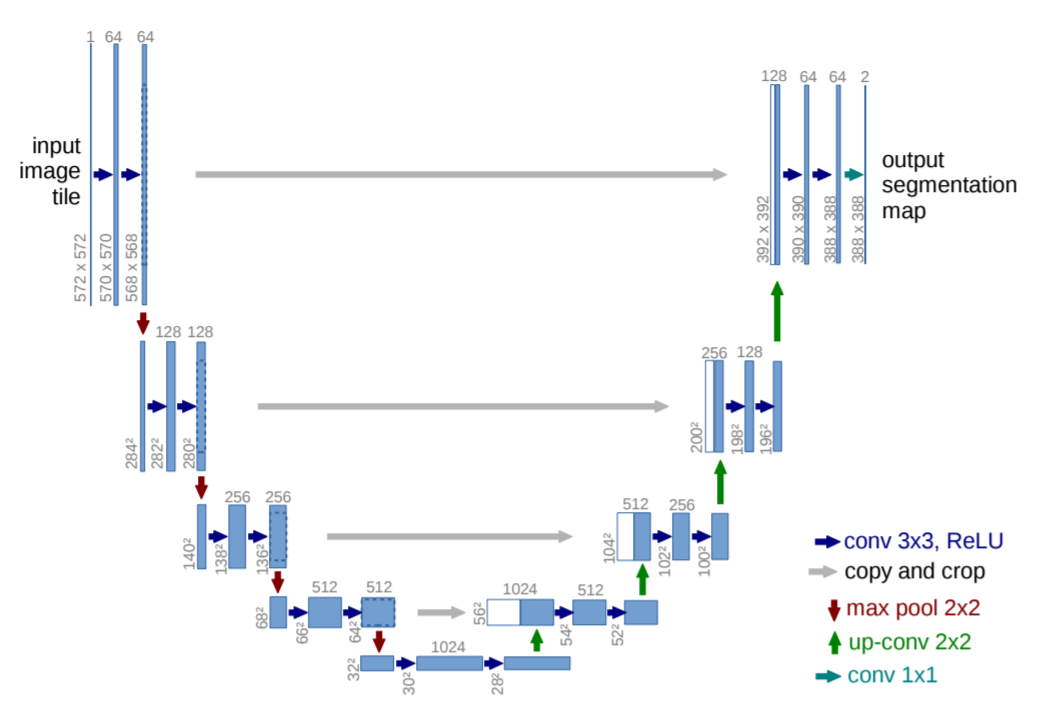
\includegraphics[width=.8\columnwidth]{report/images/UNet.png}
    \caption{
        U-Net example as described in the original paper~\cite{ronneberger2015unet}.
        Blue boxes correspond to multi-channel feature maps; the number of channels is found on top of the box, and the dimensions are at the lower left edge.
        White boxes represent copied feature maps.
    }
    \label{fig:UNetarchitecture}
\end{figure}

\subsection{Loss}\label{loss}
This is a binary problem, the pixel is either PV or no-PV. We try the following three losses:
\begin{itemize}
    \item Binary cross entropy (BCE),
    \item Weighted binary cross entropy (wBCE), and
    \item L1 loss.
\end{itemize}

The weighted binary cross entropy can be used when there is a class imbalance, which is the case here:
most pixels are no-PV. 
The formula for this loss is:
\begin{equation*}
    L = \frac{1}{N} \sum_{n=1}^N  [py_n \log(\sigma(x_n))
        + (1-y_n) \log(1-\sigma(x_n))],
\end{equation*}
where $x_n$ and $y_n$ are respectively the raw output of the model and the true class (0 or 1) for pixel $n$,
and $p$ is the weight given to the positive class. 
Setting $p>1$ increases the recall, whereas $p<1$ increases the precision.
As described in the documentation of PyTorch we set this weight as
% $\frac{\text{\#negative pixels}}{\text{\#positive pixels}}$
$\frac{\mathrm{support}(0)}{\mathrm{support}(1)}$
in the dataset.


\subsection{Training}
We train the model with different hyperparameters and choose the combination which has the best results on the validation set. In particular, we look at the following parameters:

\subsubsection{Optimizer}
We decide to try Adam~\cite{kingma2014adam} and Stochastic Gradient Descent (SGD) to train the U-Net.

\subsubsection{Effect of using no-PV images during training}
We surmise that using too few no-PV images might lead to overfitting (many false positives), while too many might incentivize the model to always predict no-PV (many false negatives).
Hence, we vary the proportion of no-PV images \textit{compared to PV images} in the train set, between 0\%, 25\% and 50\%.

\subsubsection{Loss}
We compare the three losses mentioned in \autoref{loss}.
For the weighted cross entropy loss we use a different weight depending on the percentage of no-PV images in the train set; we compute it as
$\frac{\mathrm{support}(0)}{\mathrm{support}(1)}$:

\begin{center}
    \begin{tabular}{||c | c||} 
        \hline
        Percentage no-PV & Weight for wBCE\\ [0.5ex] 
        \hline\hline
        $0\%$ & $5.13$ \\
        \hline
        $25\%$ & $6.46$ \\
        \hline
        $50\%$ & $8.10$ \\
       % [1ex] 
        \hline
    \end{tabular}
\end{center}

\subsubsection{Learning rate scheduling}
For the optimizer, the learning rate is an important factor:
small values tend to lead to a lower minimum of the loss function but very slowly and might easily get stuck in local minima, while big values lead to faster convergence but do not guarantee the best minimum.
To combine the best of both, we also use a learning rate scheduler, decreasing the learning rate as training progresses.

\subsection{Tuning threshold on probability after training model} \label{ssec:threshold}
After using a sigmoid to transform the model output into numbers in $[0,1]$, 
we still need to find a decision boundary to compare the prediction with the true label---a threshold probability $\theta$ over which a pixel is decided to be PV.
We hence perform a grid-search over thresholds between 0 and 1, computing the $F_1$-score over our validation set 
for each threshold.


As a reminder,
the $F_1$-score is computed as $2 \times \frac{\text{precision} \times \text{recall}}{\text{precision} + \text{recall}}$,
where the precision of the prediction
corresponds to $\P{\text{Pred}=1 \given \text{Label} = 1}$ while
the recall corresponds to $\P{\text{Label}=1 \given \text{Pred} = 1}$.
As such, both are susceptible to become undefined if
$\#\tl1 = 0$ or $\#\pl1 = 0$, respectively.

Since we must have no-PV images in the validation and test sets in order to faithfully represent real-world usage,
these possibilities must be accounted for.
By default, the precision and recall functions we use
can catch these errors and arbitrarily set the each value to
0 or to 1.

Setting the value to 0 in case of no-PV is not sensible,
because in this case, even if the model perfectly predicts
all pixels as 0, both precision and recall will be set to 0
(and so will the $F_1$-score).
However, setting the value to 1 also seems suboptimal, because
then we cannot make the difference between getting
a high score because PV pixels are predicted well, and just because the image is no-PV.
In both cases, the $F_1$-score is being influenced artificially in a varying way.

Another solution was then to compute precision and recall
as weighted averages, as is done with multi-class
problems.
In this case, we compute the precision and recall, once 
with PV as the positive class (so that a true positive corresponds to a pixel that is no-PV both in the predicted label and the true label) and then once with no-PV as the
positive class (so that a true positive corresponds to a pixel that is no-PV both in the predicted label and the true label).
Then, we take a weighted average of
the two, where the weights are the support of each class.
Using this method, division-by-zero issues naturally disappear.
Unfortunately, we could not interpret the results because
we tended to get a disproportionately high
precision whereas the recall was not as affected.

Finally, we decided that the best would be to \textit{concatenate all the images
in the set} and compute each metric just once.
That way, though we lose out on the statistical power
that computing for each image might bring, we are
certain that no undefined behaviour will occur, and interpretation is easier than with modified metrics.

Using this strategy, we could compute precision-recall curves and maximise the $F_1$-score. Such a precision-recall curve is shown in \autoref{fig:precision_recall}.

\subsection{Testing}
Once the best threshold is found, we use this to produce
the final model; we apply this on our test set and compute
standard classification metrics for each prediction,
using the last method presented in \autoref{ssec:threshold}.

Because the precision, recall and $F_1$-score were used
to find the best threshold, it makes sense to use other indicators for testing (the same way that using the training data for testing is not the best indicator of real-world performance).
We use the IoU loss for testing, as
it corresponds to the tightness of the overlap between
predicted and true labels.
If our task is used to estimate the total area available
for solar panels, this tightness is a very relevant metric.


\section{Results}
After selecting appropriate learning rates we choose to train the models listed in \autoref{tbl:model_parameters}.
\begin{table}
    \begin{center}
        \begin{tabular}{||c | c c c c||}
             \hline
             N\degree & Optimizer & $\%$noPV & Learning rate & Loss \\ \hline\hline
1 & ADAM & $0\% $ & $10^{-3}$ & wBCE \\ \hline
2 & ADAM & $0\% $ & $10^{-4}$ & wBCE \\ \hline
3 & ADAM & $0\% $ & $10^{-3}$ and $10^{-4}$ & wBCE \\ \hline
4 & ADAM & $25\% $ & $10^{-3}$  & wBCE \\ \hline
5 & ADAM & $25\% $ & $10^{-4}$ & wBCE \\ \hline
6 & ADAM & $25\% $ & $10^{-3}$ and $10^{-4}$ & wBCE \\ \hline
7 & ADAM & $50\% $ & $10^{-3}$ & wBCE \\ \hline
8 & ADAM & $50\% $ & $10^{-4}$ & wBCE \\ \hline
9 & ADAM & $50\% $ & $10^{-3}$ and $10^{-4}$ & wBCE \\ \hline
10 & SGD & $0\% $ & $10^{-3}$ & wBCE \\ \hline
11 & SGD & $0\% $ & $10^{-2}$ & wBCE \\ \hline
12 & SGD & $0\% $ & $10^{-2}$ and $10^{-3}$ & wBCE \\ \hline
13 & SGD & $25\% $ & $10^{-3}$ & wBCE \\ \hline
14 & SGD & $25\% $ & $10^{-2}$ & wBCE \\ \hline
15 & SGD & $25\% $ & $10^{-2}$ then $10^{-3}$ & wBCE \\ \hline
16 & SGD & $50\% $ & $10^{-3}$ & wBCE \\ \hline
17 & SGD & $50\% $ & $10^{-2}$ & wBCE \\ \hline
18 & SGD & $50\% $ & $10^{-2}$ and $10^{-3}$ & wBCE \\ \hline
19 & ADAM & $0\% $ & $10^{-3}$ and $10^{-4}$ & BCE \\ \hline
20 & ADAM & $25\% $ & $10^{-3}$ and $10^{-4}$ & BCE \\ \hline
21 & ADAM & $50\% $ & $10^{-3}$ and $10^{-4}$ & BCE \\ \hline
22 & ADAM & $0\% $ & $10^{-3}$ and $10^{-4}$ & L1 \\ \hline
23 & ADAM & $25\% $ & $10^{-3}$ and $10^{-4}$ & L1 \\ \hline
24 & ADAM & $50\% $ & $10^{-3}$ and $10^{-4}$ & L1 \\ \hline
        \end{tabular}
    \end{center}
    \caption{Hyperparameter combinations for the different models we consider. We write two values for the learning rate, when we use learning rate rescheduling. 
    }
    \label{tbl:model_parameters}
\end{table} 

We notice that rescheduling the learning rate during the training only once after 50 epochs gives the best results.
We also notice that when rescheduling, we need to shorten the training to 80 epochs to avoid overfitting,
whereas with a constant learning rate we train for 100 epochs to have the best results before overfitting.

Each model is run on a validation set to perform a grid-search of the best threshold,
and the model is then applied with that threshold to a test set.
Various standard classification metrics are computed and collected in \autoref{tbl:test_results}.

\begin{table}
    \begin{center}
        \begin{tabular}{||c | c c c c||}
             \hline
             N\degree & Jaccard (IoU) & $F_1$-score & Precision & Recall \\ \hline\hline
\textbf{21} & \textbf{0.6223} & \textbf{0.7672}  & \textbf{0.7491} & \textbf{0.7862} \\ \hline
 4 & 0.5999 & 0.7499 & 0.7047 & 0.8013 \\ \hline
 6 & 0.5921 & 0.7438 & 0.6939 & 0.8015 \\ \hline
 7 & 0.5862 & 0.7391 & 0.7339 & 0.7444 \\ \hline
 8 & 0.5834 & 0.7369 & 0.6716 & 0.8164 \\ \hline 
 9 & 0.5781 & 0.7327 & 0.6742 & 0.8022 \\ \hline 
20 & 0.5762 & 0.7311 & 0.6932 & 0.7735 \\ \hline
15 & 0.5685 & 0.7249 & 0.6707 & 0.7887 \\ \hline
 2 & 0.5659 & 0.7228 & 0.6542 & 0.8075 \\ \hline
22 & 0.5609 & 0.7186 & 0.6919 & 0.7476 \\ \hline
18 & 0.5493 & 0.7091 & 0.6493 & 0.7810 \\ \hline
19 & 0.5472 & 0.7073 & 0.6550 & 0.7688 \\ \hline
23 & 0.5338 & 0.6961 & 0.6650 & 0.7303 \\ \hline
14 & 0.5265 & 0.6898 & 0.6149 & 0.7856 \\ \hline
24 & 0.5243 & 0.6879 & 0.6530 & 0.7268 \\ \hline
 3 & 0.5159 & 0.6807 & 0.5951 & 0.7949 \\ \hline
 1 & 0.4868 & 0.6548 & 0.5479 & 0.8137 \\ \hline
 5 & 0.4766 & 0.6455 & 0.5629 & 0.7566 \\ \hline
12 & 0.4703 & 0.6397 & 0.5533 & 0.7581 \\ \hline
17 & 0.4570 & 0.6273 & 0.5915 & 0.6678 \\ \hline
16 & 0.4026 & 0.5741 & 0.5190 & 0.6422 \\ \hline
11 & 0.3841 & 0.5550 & 0.4453 & 0.7364 \\ \hline
13 & 0.3471 & 0.5153 & 0.4583 & 0.5885 \\ \hline
10 & 0.2351 & 0.3806 & 0.2745 & 0.6207 \\ \hline


        \end{tabular}
    \end{center}
    \caption{Test results for all models, each with its best threshold according to $\arg\max F_1(\theta)$. Sorted according to the IoU (Intersection-over-Union).
    }
    \label{tbl:test_results}
\end{table}

We choose the model 21 as the best model because it has the best IoU and $F_1$-score.
The train and validation error during training are shown in \autoref{fig:train_validation_errors}.
We see that there are some peaks but their frequency and intensity decreases after the rescheduling after 50 epochs. This suggests that using the learning rate scheduling was a good idea. \autoref{fig:precision_recall} shows the precision-recall curve and highlights the point that has been chosen as a threshold (0.37), giving the results shown in \autoref{tbl:test_results}.



\begin{figure}
\centering
    \begin{minipage}[b]{.45\columnwidth}
        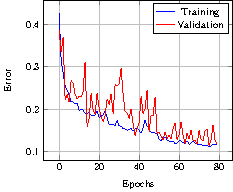
\includegraphics[width=\columnwidth]{report/images/plots/train_val_errors.pdf}
        \caption{Train and validation errors during training of the model N\degree 21.}
        \label{fig:train_validation_errors}
    \end{minipage}\quad
    \begin{minipage}[b]{.45\columnwidth}
        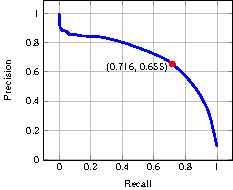
\includegraphics[width=\columnwidth]{report/images/plots/prec_rec.pdf}
        %\usepackage{standalone}

\begin{tikzpicture}
\begin{axis}[
  xlabel={Recall},
  ylabel={Precision},
  grid=major,
  height=5cm,
  width=\columnwidth,
]
  \addplot [blue] table [x=recall_mid, y=precision_mid] {prec_rec_f1_21.txt};
  % Best threshold is 0.370
\end{axis}
\end{tikzpicture}

        %\tikzsetnextfilename{prec_rec} % Nom du fichier de sortie de la figure
	    %\usepackage{standalone}

\begin{tikzpicture}
\begin{axis}[
  xlabel={Recall},
  ylabel={Precision},
  grid=major,
  height=5cm,
  width=\columnwidth,
]
  \addplot [blue] table [x=recall_mid, y=precision_mid] {prec_rec_f1_21.txt};
  % Best threshold is 0.370
\end{axis}
\end{tikzpicture}
 % Source TikZ dans un fichier annexe, pour la lisibilité
        \caption{Precision-recall curve of model N\degree 21. Red dot indicates best threshold.}
        \label{fig:precision_recall}
    \end{minipage}
\end{figure}

\begin{figure}[tbp]
    \centering
    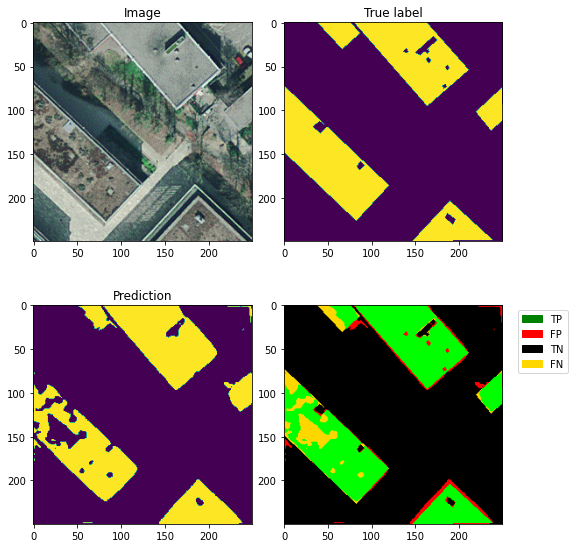
\includegraphics[width=.9\columnwidth]{report/images/prediction.png}
    \caption{Prediction of model N\degree 21 on an image from the Test set using a threshold of 0.37.}
    \label{fig:prediction}
    \vspace{-0.5cm}
\end{figure}

\section{Discussion}
We convince ourselves that this model works well by looking at the predictions it makes. \autoref{fig:prediction} shows the prediction of the model on a test image.
We see that the model recognizes roofs really well and manages to exclude many obstacles and solar panels. However it has more trouble spotting small obstacles on the roof, and differentiating a roof from a flat ground surface.
From our experience in labelling the data, we can note that the scenarios mentioned above can be hard to label for humans as well. Also, it often happens that the model makes better predictions than humans, so more accurate labelling could increase its performance.

We used a test set corresponding to the real distribution of PV and no-PV images, so that our model stays as general as possible. Another model might give better results on a preprocessed dataset with less no-PV images.

In general, we see that ADAM outperforms SGD.
We observe that using the L1 loss is consistently the worst and surprisingly, using the weighted version of BCE does not always give the best results.
This might be due to the fact that we are basing our predictions on a threshold that we calculate once the U-Net is ready, independently of the loss used during training.
By doing so, we ensure that even models trained with an unbalanced loss, that would tend to more easily predict no-PV pixels, can give meaningful results by using a low threshold.
Indeed, we see that models trained with BCE have have significantly lower decision thresholds.
We also note that training with more no-PV images generally yields better results.

Depending on the use case for which this model would be used, it can make more sense to use a different metric to set the threshold value for decisions.
If the user wants to minimize the false negative rate, in order to make sure not to underestimate the available area for solar panels, we would suggest to decrease the threshold and vice versa.

Because we are using a shared GPU from the lab running other experiments, we are limited in our computational resources, but more fine-tuning of the hyperparameters, especially the learning rate and its scheduler, could further increase the performance of our model.

\section{Conclusion}
In this project we propose a model to detect rooftop solar panels in aerial images based on a U-Net. When applied on a test set of images that have not been preprocessed (e.g. removing no-PV images), we get a $F_1$-score of $0.77$ and an IoU score of 0.62. 
In our analysis, we fix the decision threshold for this model to $0.37$ but we also give insights on how to change this value depending on the final use of the model.
The U-Net could give better performances with more labelled data. We thus provide a tool that enables to label new data more easily.

\section*{Acknowledgements}
We would like to thank Roberto Castello and Simon Roquette from the Solar Energy and Building Physics Lab for their guidance and valuable advice during this project.
%\bibliographystyle{ieeetr}
%\bibliography{report}
\printbibliography


\end{document}
